%pme2360
\section{12.44}

% \begin{figure}[h]
% \begin{center}
% 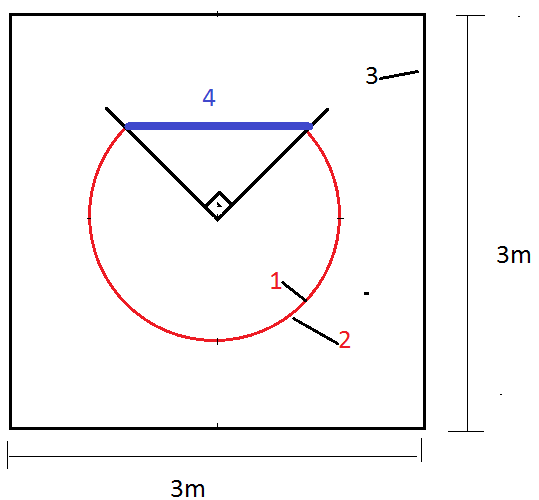
\includegraphics[scale=0.28]{./fig/1.png}
% \caption{\label{fig:1}1} 
% \end{center}
% \end{figure}

\myfig[scale=.28]{figPME2360-20111116-01}{}

\subsection{a) emissividade total e absorvidade total}

Quer que calculemos $\varepsilon$ (poder emissivo espectral de um corpo negro) e $\alpha$


\begin{verbatim}
Emissividade total computa a radiação emitida por toda uma superfície
poder emissivo espectral de um corpo negro
emissividade também depende da temperatura da superfície
3 niveis da lei de kirchhoff
\end{verbatim}

\[\varepsilon = \frac{\int _{0} ^{\infty} {\varepsilon(\lambda)E_{CN,\lambda(\lambda ,T)}}d\lambda}{E_{CN}(T)}\]

\[\alpha = \frac{\int _{0}^{\infty}\alpha _{\lambda}G(\lambda)d\lambda }{G}\]

\[
\varepsilon = \frac{\int _{0}^{1\mu m}\varepsilon _{\lambda}E_{CN,\lambda}}{E_{CN}(T)} + \frac{\int _{1}^{3\mu m}\varepsilon _{\lambda}E_{CN,\lambda}}{E_{CN}(T)} + \frac{\int _{3}^{1\infty}\varepsilon _{\lambda}E_{CN,\lambda}}{E_{CN}(T)}
\]

\[
\varepsilon = \varepsilon _{1 \rightarrow 3} \frac{\int _{0}^{1\mu m}\varepsilon _{\lambda}E_{CN,\lambda}}{E_{CN}(T)} +  \varepsilon _{3 \rightarrow \infty} \frac{\int _{1}^{3\mu m}\varepsilon _{\lambda}E_{CN,\lambda}}{E_{CN}(T)} 
\]

\[
\varepsilon = \varepsilon _{1 \rightarrow 3} \times F_{1 \rightarrow 3\mu m} +  \varepsilon _{3 \rightarrow \infty} \times F_{3 \rightarrow  \infty}
\]

Em que

\begin{itemize}
\item $ F_{1 \rightarrow 3\mu m}$ = $F_{0 \rightarrow 3} - F_{0 \rightarrow 1}$
\item $ F_{3 \rightarrow \infty}$ = $1 - F_{0 \rightarrow 3}$
\end{itemize}


Consultar a tabela 12.1

\[
\lambda T = 1 \mu m \times 400K = 400 \mu mK \rightarrow F_{0 \rightarrow 1\mu m} = 0.000000
\]

\[
\lambda T = 3 \mu m \times 400K = 1200 \mu mK \rightarrow F_{0 \rightarrow 3\mu m} = 0.002134
\]

\[
\varepsilon = 0.7 \times (0.002134 - 0.000000)+0.5 \times (1-0.002134)
\]

\[\varepsilon = 0.500\]

% \begin{figure}[h]
% \begin{center}
% 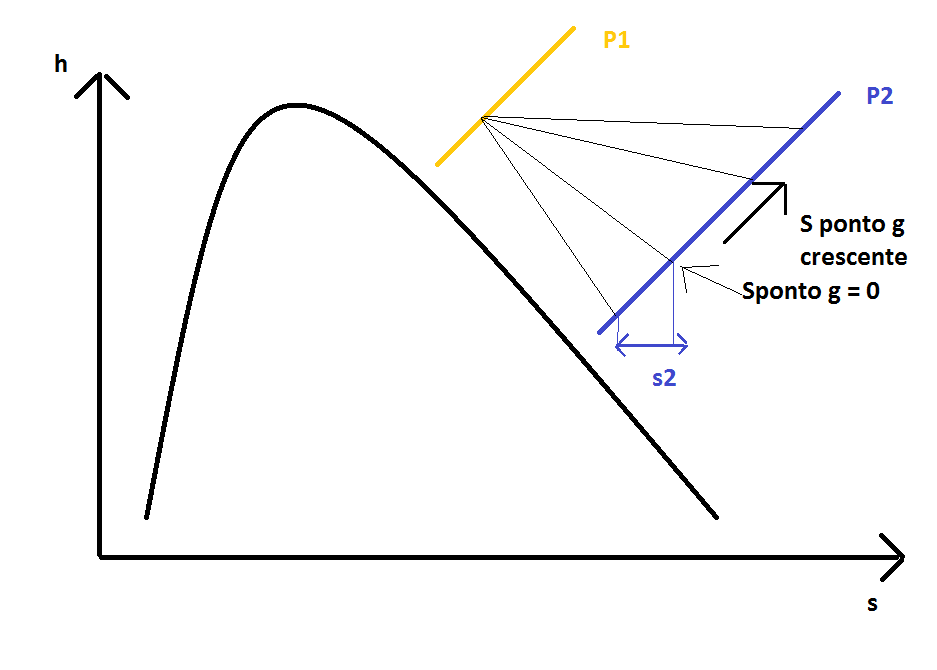
\includegraphics[scale=0.28]{./fig/2.png}
% \caption{\label{fig:2}2} 
% \end{center}
% \end{figure}

\myfig[scale=.28]{figPME2360-20111116-02}{}

Difusa:

\begin{itemize}
\item $\varepsilon _{\lambda} = \alpha _{\lambda}$
\item $G(\lambda) = E_{CN,\lambda}(T_{f})$
\end{itemize}

Em que $E_{CN,\lambda}$ é a do forno.
\[G = E_{CN}(T_{f})\]

\[
\alpha = \alpha _{1 \rightarrow 3}F_{1 \rightarrow 3} + \alpha _{3 \rightarrow \infty}F_{3 \rightarrow \infty}
\]

\[
\lambda T = 1 \mu m \times 2000K = 2000 \mu mK \rightarrow F_{0 \rightarrow 1\mu m} = 0.066728
\]

\[
\lambda T = 3 \mu m \times 2000K = 6000 \mu mK \rightarrow F_{0 \rightarrow 3\mu m} = 0.737818
\]

\[
\alpha = 0.7 \times (0.737818 - 0.066728)+0.5 \times (1-0.0.737818)
\]

\[\alpha = 0.6\]


\subsection{b) refletida}

\[(1-\alpha)G=0.4 \times \sigma \times 2000^{4} = 3.621 \times 10 ^{5} W/m^{2}\]
Líquido:

\[q'' = \alpha G - \varepsilon E_{CN}(T_{s})\]
Em 	que G = $E_{CN}(T_{f})$

\[q'' = \alpha \sigma T_{f}^{4} - \varepsilon  \sigma T_{s}^{4}\]
\[q'' = 5.45 \times 10^{5} W/m^{2}\]

\subsection{c)$E_{\lambda=2 \mu m}(T_{s}) = ?$  }


\[E_{\lambda , CN}\]

\[
E_{\alpha} = 2 \mu m = \varepsilon _{\lambda} = 2 \mu E_{CN,\lambda}
\]

Consultar a tabela 12.1:\ \ \ \ \ 
\begin{tabular}{|c|c|}
\hline 
$\lambda T$ & $\frac{I_{\lambda , CN}}{\sigma T^{5}}$ \\ 
\hline 
• & • \\ 
\hline 
\end{tabular} 

\[E_{CN,\lambda} = \pi I_{\lambda,CN}\]
Em que a unidade de $E_{CN,\lambda}$ é $W/(m^{2} \mu m)$

Para $\lambda T = 2 \times 400 = 800 \mu mK$

\[
\frac{I_{\lambda , CN}}{\sigma T^{5}\footnote{400 K}} = 0.991126 \times 10^{-7}
\]

\[
I_{\lambda , CN} = 0.0575 \frac{W}{m^{2} \mu m }
\]

\[E_{\lambda=2 \mu m} = 0.7 \times \pi \times  0.0575 = 0.126 \frac{W}{\mu m m^{2}}\]

\subsection{d) $\lambda _{1/2} = ?$}

Para$ F_{0 \rightarrow \lambda 1/2} = 0.5$.
Da tabela,

\[
\lambda T = 4100 \mu m K
\]
Onde T = 400 K
\[\lambda _{1/2} = 10.3 \mu m\]

\pagebreak

\section{13.119}

% \begin{figure}[h]
% \begin{center}
% 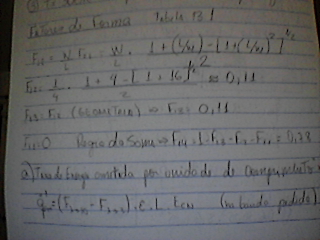
\includegraphics[scale=0.28]{./fig/3.png}
% \caption{\label{fig:3}3} 
% \end{center}
% \end{figure}

\myfig[scale=.28]{figPME2360-20111116-03}{}

% \begin{figure}[ht]
% \subfigure[4]{
% \label{fig:4}
% 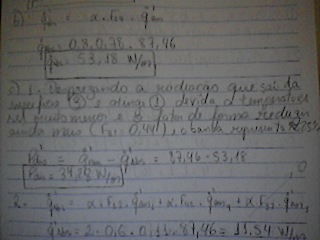
\includegraphics[scale=0.26]{./fig/5.png}
% }
% \subfigure[5]{
% \label{fig:5}
% 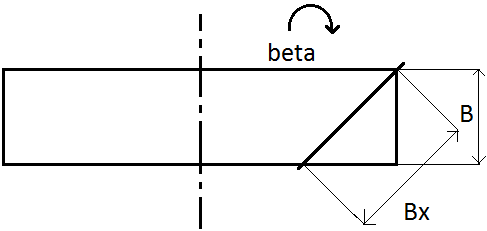
\includegraphics[scale=0.26]{./fig/4.png}
% }
% \caption{\label{fig:6}}
% \subref{fig:4} ,\subref{fig:5}
% \end{figure}

\myfig[scale=.28]{figPME2360-20111116-05}{}

\myfig[scale=.28]{figPME2360-20111116-04}{}

\[\frac{1}{A_{1}} \left[  \frac{1-\varepsilon_{1}}{\varepsilon_{1}} + \frac{1}{F_{12}=1  } + \frac{1-\varepsilon _{2}}{\varepsilon _{2} A_{2}/A_{1}} \right]\]

\begin{verbatim}
Falta a energia que sai do circuito. 3 superfícies equivalem a 3 nós. 
Qual a superfície do 3º nó?
\end{verbatim}